\section{Fundamentals}
\label{sec:fundamentals}
This chapter will cover the basics of this thesis beginning with a short introduction in \gls{see} in section \ref{sec:see}.
Section \ref{sec:code_cities} will continue with giving insight on \glspl{city}. 
In the end of this chapter, section \gls{unity} will be about \gls{unity} and the core functions that will be used in this thesis.

\subsection{SEE}
\label{sec:see}
The \gls{see} project aims to connect people regardless of space in a virtual room to analyze code structure. 
The Unity based project uses various types of code visualization (\cite{koschke}, \cite{DBLP:conf/iwsc/KoschkeS21}). 
One scenario uses the metaphor of cities to illustrate the code structure of an application.
An example of such an \gls{city} can be seen in figure \ref{fig:see_example}.
Such city graphs can be imported from \gls{glx} files.
Elements that represent building will be called \glspl{node} and underlying platform will be called \gls{plane}.

In the current state of the SEE project the virtual room can be accessed with VR glasses or a desktop computer.
This thesis aims to add an implementation of \gls{see} for \gls{android} devices.
This shall help developers to collaborate on software projects as freely as possible.
\begin{figure}[htb]
    \centering
    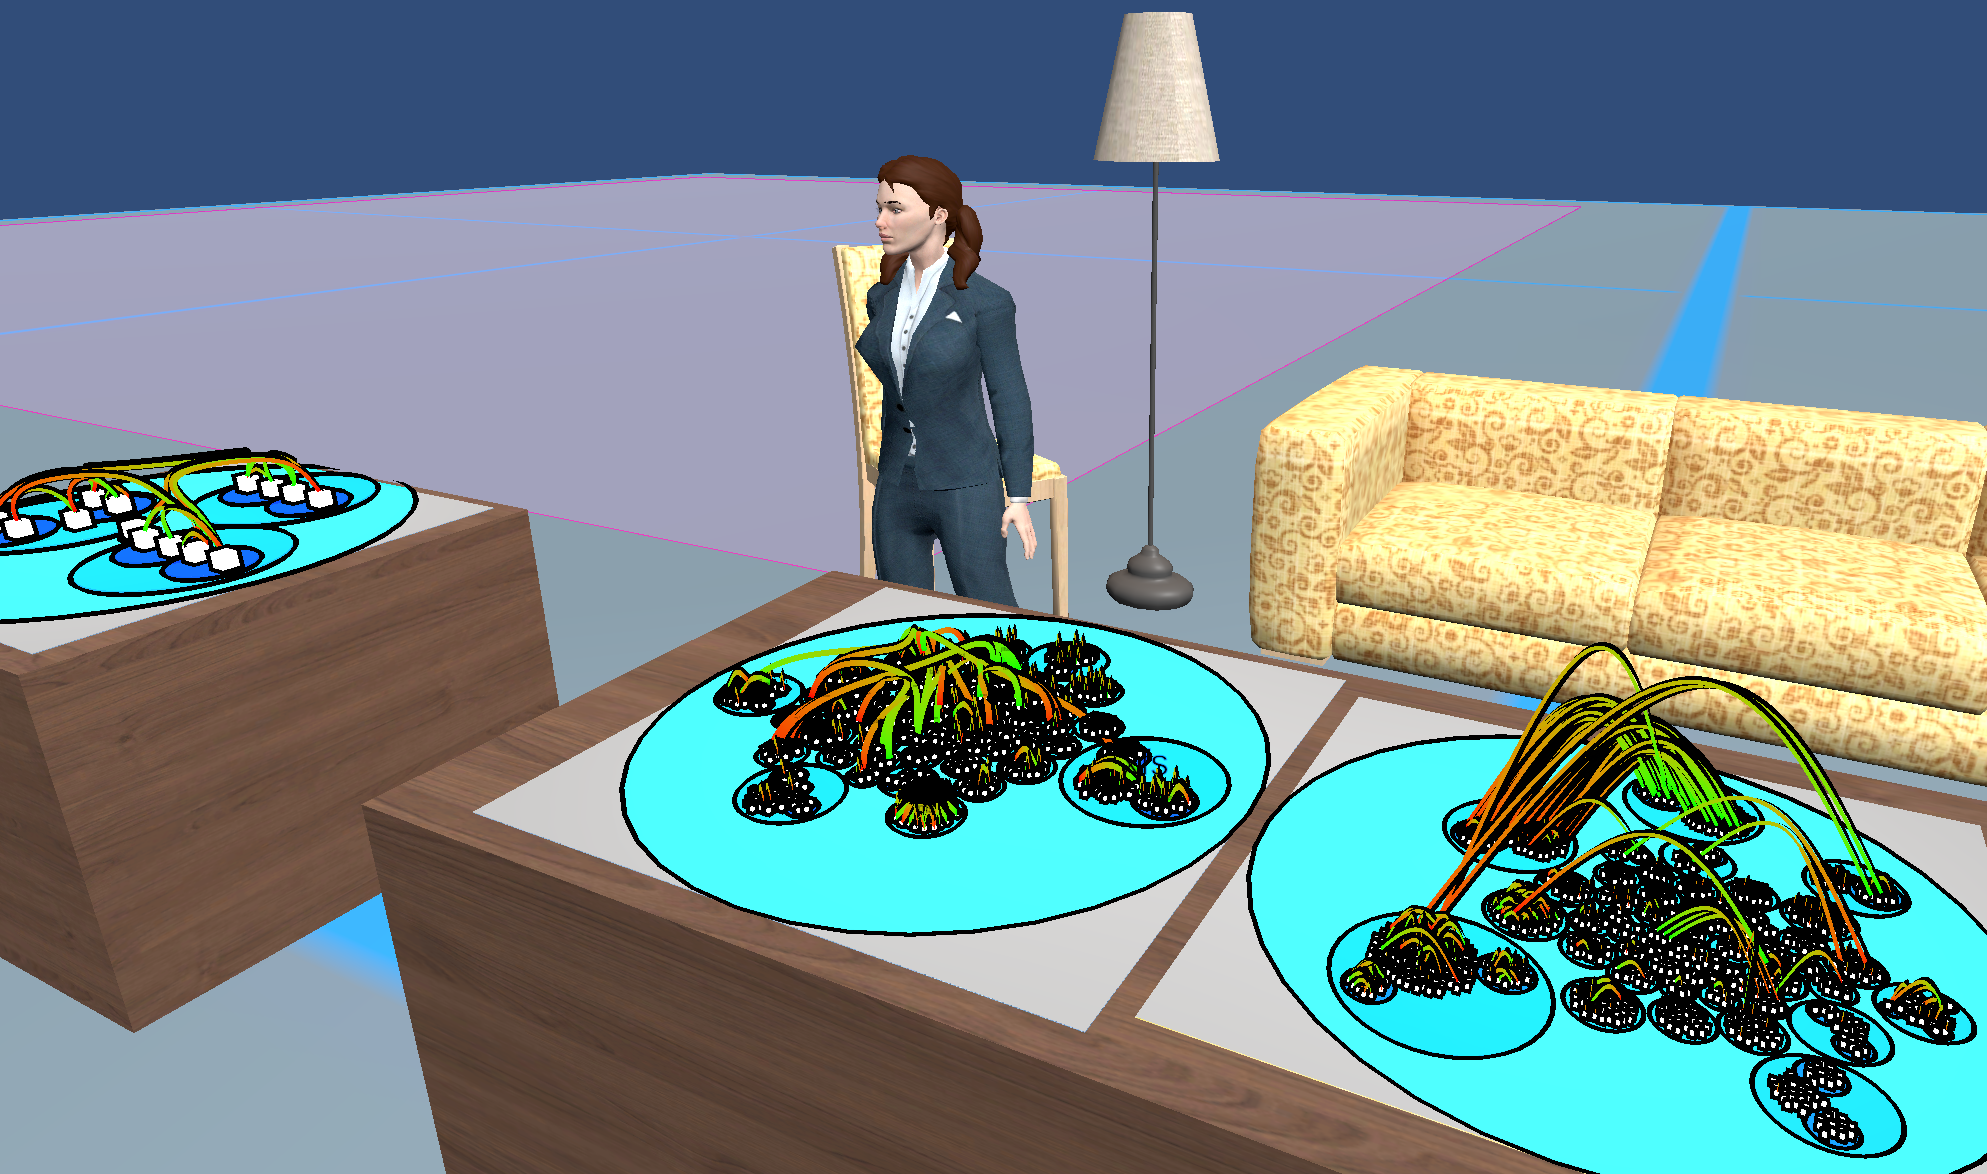
\includegraphics[width=1\textwidth]{Fundamentals/img/SEE.png}
    \caption{An example of \gls{see} used for the user study in chapter \ref{section:evaluation}}
    \label{fig:see_example}
\end{figure}

\subsection{Code Cities}
\label{sec:code_cities}
A \gls{city} is an approach of visualizing software projects.
An example of a \gls{city} by \cite{wettel2007visualizing} can be seen in figure \ref{fig:city_example}.
Since the representation is three-dimensional many metrics can be visualized in a single \gls{city}.
Code Cites could use, as an example, the metrics number of classes as building height, number of attributes as base size and the and the nesting level of a package as the building color (\cite{wettel2008visual}).
The \gls{city} provides an overview of the represented system and by walking around it in \gls{see} the user can get an idea of the structure of the represented system.
On challenge of representing large code bases is the overwhelming amount of information.
Therefore, using metaphors as the \gls{city} aims to avoid overwhelming the user with too much abstract information (\cite{Wettel2008}).
\begin{figure}[htb]
    \centering
    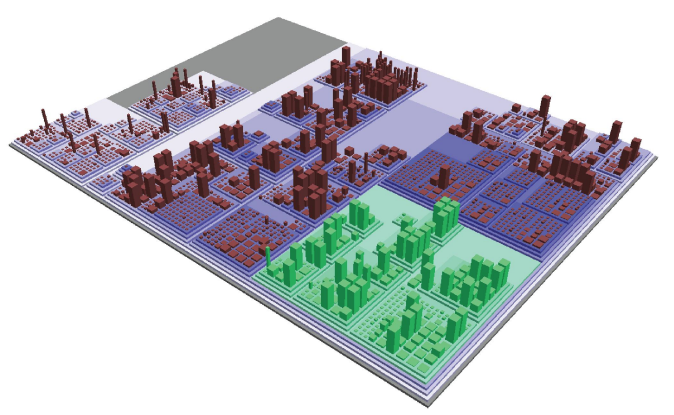
\includegraphics[width=1\textwidth]{Fundamentals/img/code_city.png}
    \caption{An example for a \gls{city} by \cite{wettel2007visualizing}}
    \label{fig:city_example}
\end{figure}

\subsection{Unity}
\gls{unity} is a cross-platform game engine that has been released in June 2005 as \textit{Unity 1.0}.
The engine is not only popular for games but also for other industries regarding architecture, automotive or film\footnote{https://unity.com/ (last visited: 22.06.22, 2:39)}.
\gls{unity} started to become successful with its launch in the Apple App Store. 
This is due to the growing popularity of mobile video games and \gls{unity} being on of only few game engines that are optimized for Apple.
The game engine grew ever since and has grown its support for multiplatform development (\cite{nicoll2019unity}).

\subsubsection{Ray Casting}
\label{sec:ray}
Ray casting is basic computer graphics rendering algorithm. 
Rays are cast to determine on their path what can be seen be the camera perspective. 
In the example of figure \ref{fig:ray_example} a local camera coordinate system can be seen.
The lines from the origin on the right are rays that determine the view plane of $z=0$.
\begin{figure}[htb]
    \centering
    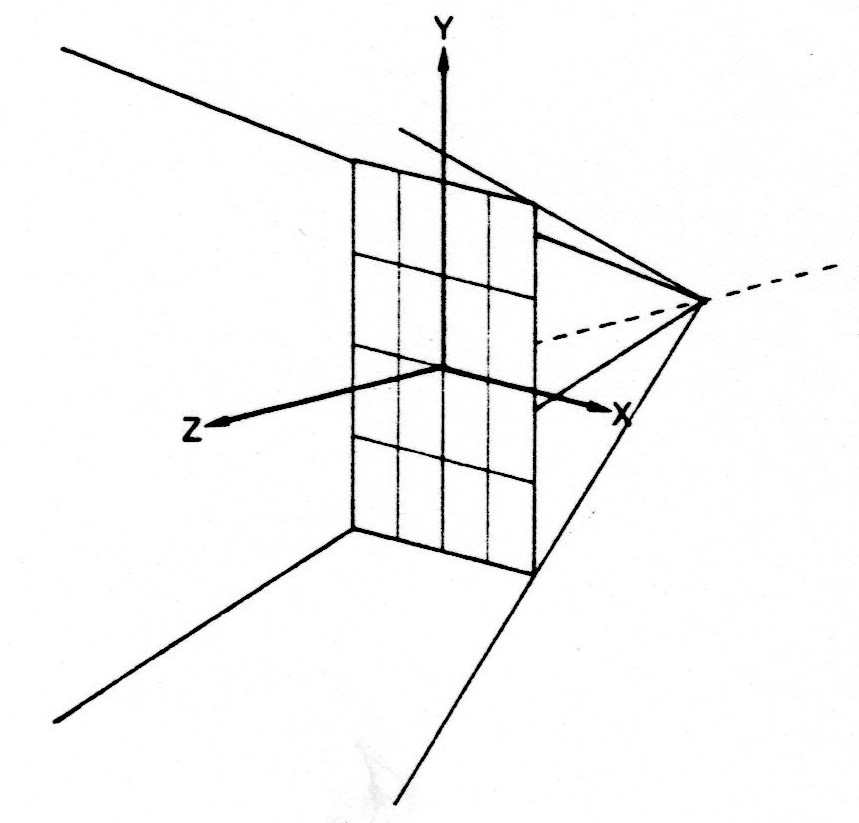
\includegraphics[width=1\textwidth]{Fundamentals/img/ray_casting.jpg}
    \caption{Camera's local coordinate system by \cite{roth1982ray}}
    \label{fig:ray_example}
\end{figure}

Ray casting will also be used to detect the closest object from a certain point on the camera's perspective.
For example objects will often be selected by touch and to determine with object is touched ray casting is needed.
Therefore, a ray will be cast from the center of the touch input and call be the closest object. 
This could also be used to determine if a touch input is on a \gls{city} to allow rotating or moving interactions. 

\subsubsection{Debugging and Testing}
Building another version of a consisting application can take a lot of testing.
Testing in \gls{unity} for \gls{android} applications can be escalated in three steps. 
Debugging always works in combination with the \textit{Microsoft Visual Studio}\footnote{visualstudio.microsoft.com/ (last visited: 24.06.22, 0:12)} debugger, an \gls{ide} for multiple coding languages including \textit{C\#}.

The first and easiest method can be done directly in the \gls{unity} Editor by using the core feature \textit{Play Mode}.
In \textit{Play Mode} the project starts and builds as it would in a final build.
Any changes made in will not be saved and will be reset after leaving \textit{Play Mode}.
However, the building time in the \textit{Play Mode} is much faster than the actual \gls{android} build.
Unfortunately touch input can not be tested on a desktop computer, but the \textit{Play Mode} suffices for testing UIs or other basic changes. 

\begin{figure}[htb]
    \centering
    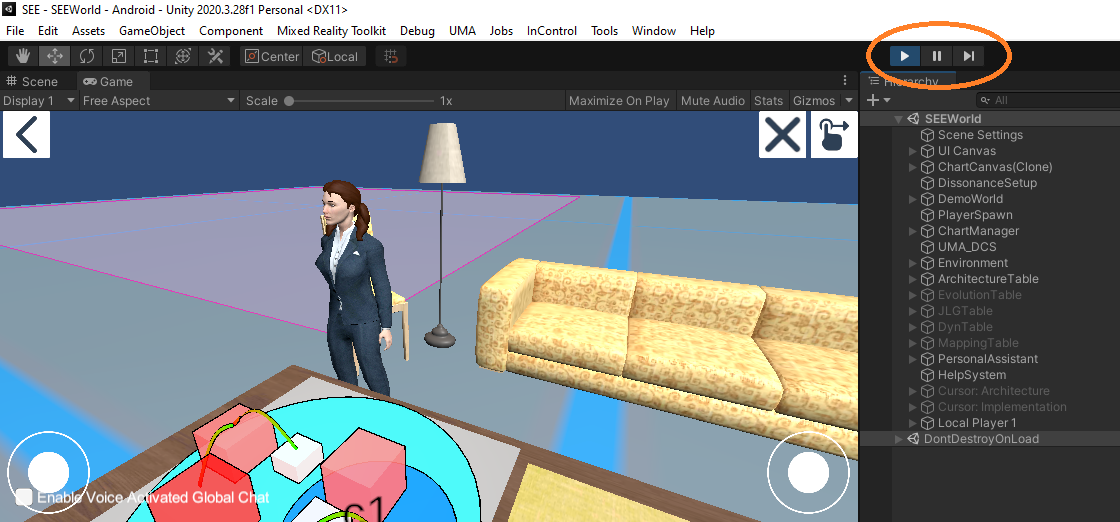
\includegraphics[width=1\textwidth]{Fundamentals/img/play_mode.png}
    \caption{The \textit{Play Mode} can be entered by pressing play at the marked spot}
    \label{fig:play_mode}
\end{figure}

However, if actions with touch input need to be tested, the second method is suitable.
Therefore, \gls{unity} provides the app \textit{Unity Remote}\footnote{https://docs.unity3d.com/Manual/UnityRemote5.html (last visited: 24.06.22, 0:14)}.
The app can be connected via USB with the \gls{unity} Editor.
After hitting the play button the \gls{scene} will also be displayed on the connected device and also take input.
Besides touch input other factors for a mobile application like the accelerometer, gyroscope or the camera can be tested. 
The application however will be build on the desktop computer and not on the \gls{android} device. 

To test the application for example for bugs that cause a crash on some \gls{android} devices the application has to be build and installed on the device.
The device can then be connected with the \gls{ide} via Wi-Fi or USB. 
\gls{unity} also provide an option to let the built application wait for a connection with the \gls{ide}, since the connection can take some time.
This however is more time-consuming than the other to methods. 
An \gls{unity} \gls{android} build can take depending on the project size more than five minutes. 
It should therefore only be a last option and only be used to debug concerns regarding the devices hardware constrains. 
